\documentclass[12pt]{article}

\usepackage[top=0.75in,bottom=0.75in,left=0.5in,right=0.5in]{geometry}
\usepackage{amsmath,amssymb,multirow,graphicx,wrapfig}

\newcommand{\bee}[1]{\begin{equation} #1 \end{equation}}
\newcommand{\baa}[1]{\begin{eqnarray} #1 \end{eqnarray}}
\newcommand{\bees}[1]{\begin{equation*} #1 \end{equation*}}
\newcommand{\baas}[1]{\begin{eqnarray*} #1 \end{eqnarray*}}

\newcommand{\pd}[2]{\ensuremath{\frac{\partial #1}{\partial #2}}}
\newcommand{\dd}[2]{\ensuremath{\frac{d #1}{d #2}}}

\newcommand{\bu}{{\mathbf u}}
\newcommand{\bF}{{\mathbf F}}


\title{2D Conservative Upwinding Scheme}
\author{Bree Cummins}

\begin{document}
\maketitle

\section{Introduction}
We want to numerically solve the 2D advection equation 
\bees{
\pd{C}{t} + \nabla \cdot \bF = 0, 
}
where $C(x,y,t)$ is the concentration of a substance and the flux is the product of concentration and a prescribed velocity: $\bF = \bu(x,y,t) C(x,y,t)$. For later work, it is convenient to denote the components of velocity by $\bu = (u,v)$, and those of the flux by $\bF = (f,g) = (uC,vC)$. 

\begin{wrapfigure}{l}{3.0in}
	\begin{center}
	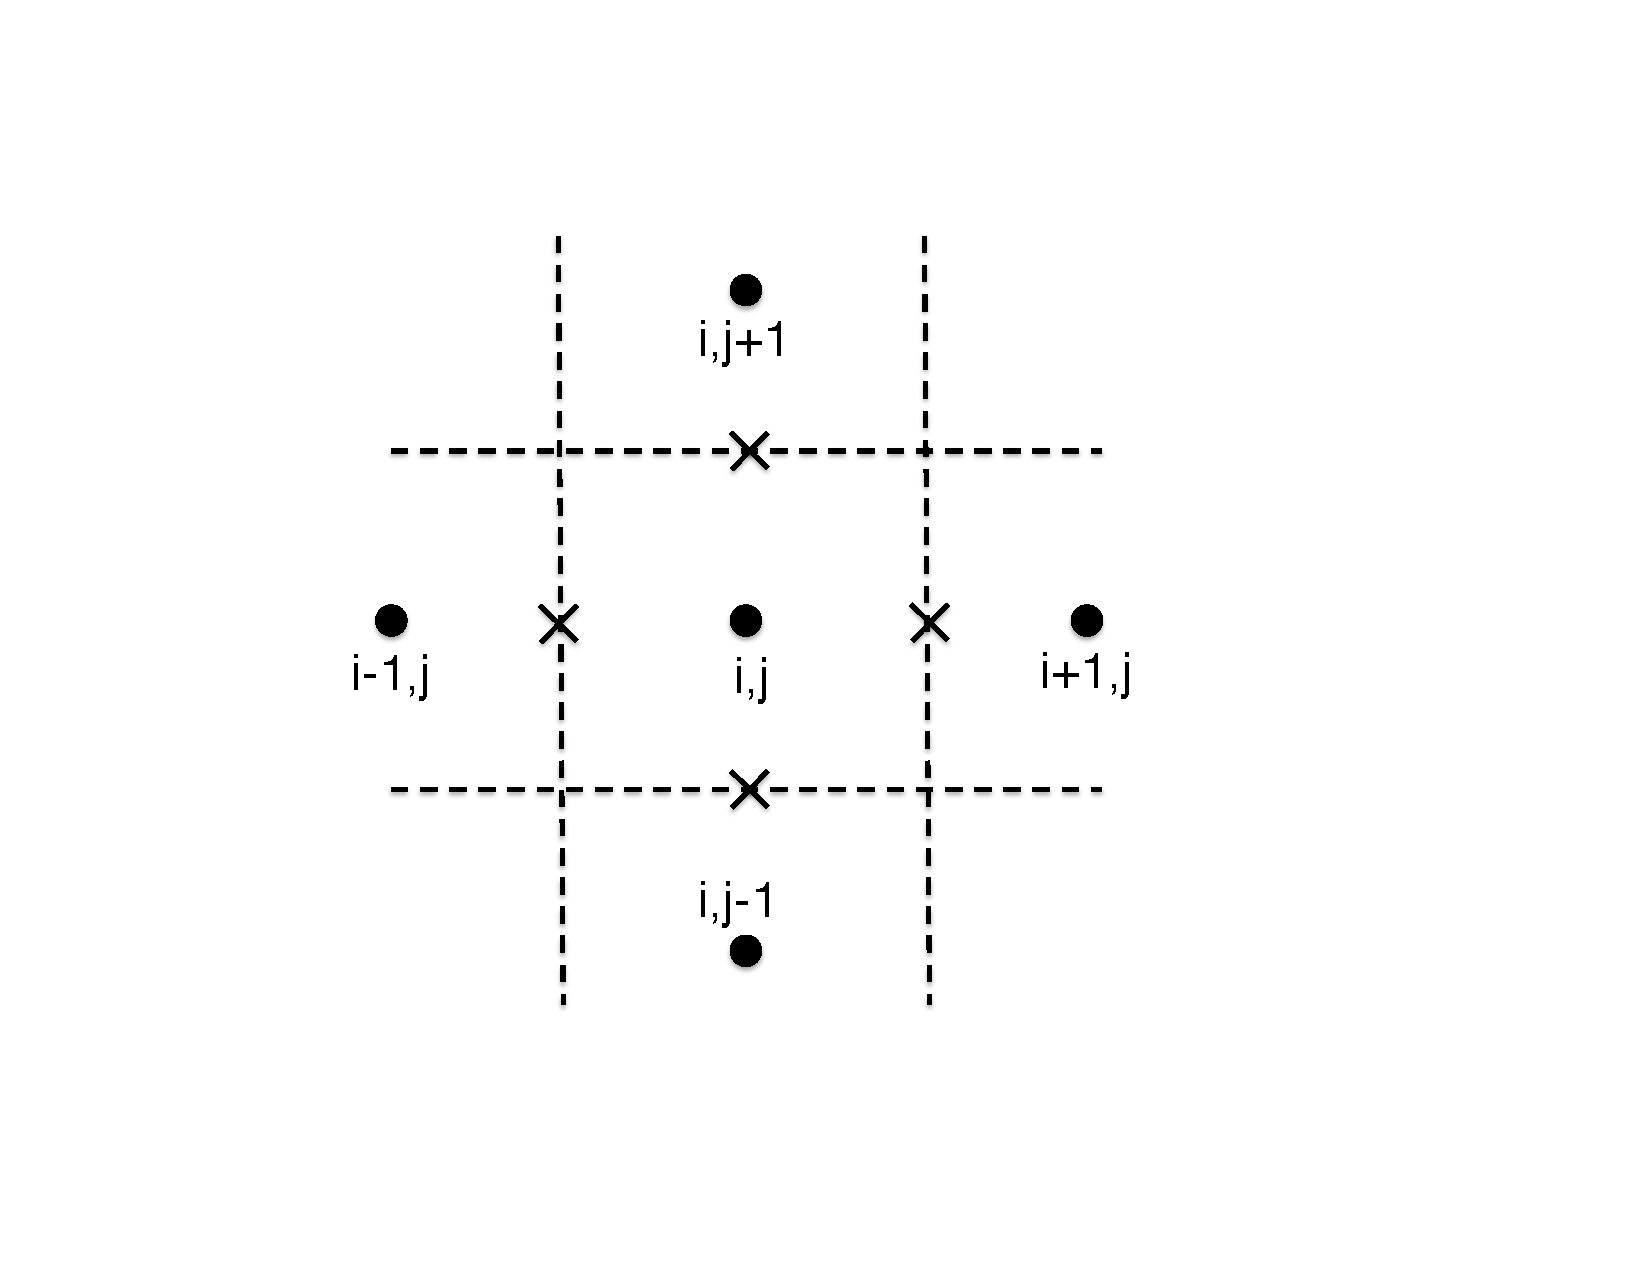
\includegraphics[width=3.0in]{figures/gridschematic.pdf}
	\caption{A schematic of a typical cell with neighbors in all directions. The x's denote an offset grid that is used in the conservative upwinding scheme.} \label{grid}
\end{center}
\end{wrapfigure}

We will consider a solution over the square domain, $[0,1] \times [0,1]$, where the boundary conditions enforce zero net flux. We discretize the domain into $N$ cells on a side, indexed by $i = 1,\dotsc,N$ in the $x$ coordinate and by $j$ in the $y$ coordinate. We track the concentration and velocity at the cell centers, so that $C_{ij}$ refers to the concentration value at the center of the $ij$-th cell. 

Let $\Delta x$ and $\Delta y$ denote grid spacing in the $x$ and $y$ directions. If the $ij$-th value of $\nabla \cdot \bF$ is approximated using center differences across the cell centers
\bees{
(\nabla \cdot \bF)_{ij} \approx \frac{f_{i+1,j} - f_{i-1,j}}{2\Delta x} + \frac{g_{i,j+1} - g_{i,j-1}}{2\Delta y},
}
then the numerical solution is unstable. This is because information travels along characteristics in the domain, and at the edge of an advancing front, center differences average between values both before and after the front. This results in accumulating error. 

To avoid this issue, computational scientists use ``upwinding" schemes that calculate derivatives using values from the direction of the prevailing velocity. However, not all upwinding schemes are guaranteed to conserve the amount of concentration in the domain even with no net flux boundary conditions. We want to choose our upwinding scheme so that concentration is conserved:
\bees{
\pd{}{t}\int_{0}^{1}\int_{0}^{1} C \, dx \, dy = 0.
}

\section{Conservative upwinding}

Instead of calculating derivatives across cell centers, we will use approximate values at cell edges (the offset grid of x's in Fig.~\ref{grid}):
\bee{
(\nabla \cdot \bF)_{ij} \approx \frac{f_{i+1/2,j} - f_{i-1/2,j}}{\Delta x} + \frac{g_{i,j+1/2} - g_{i,j-1/2}}{\Delta y}, \label{consup} 
}
where $f_{i+1/2,j} = u_{i+1/2,j}C_{i+1/2,j}$, etc. In order to approximate velocities at the edge midpoints, we
average over adjacent cells:
\\
\begin{center}
\begin{tabular}{cc}
$u_{i+1/2,j} \equiv \frac{1}{2} \left( u_{ij} + u_{i+1,j} \right)$ & $u_{i-1/2,j} \equiv \frac{1}{2} \left( u_{i-1,j} + u_{i,j} \right)$ \\
$v_{i,j+1/2} \equiv \frac{1}{2} \left( v_{ij} + v_{i,j+1} \right)$ & $v_{i,j-1/2} \equiv \frac{1}{2} \left( v_{i,j-1} + v_{i,j} \right)$ .
\end{tabular}
\end{center}
Then we choose the concentration at the edge midpoints to be one of the adjacent centers depending on the sign of the averaged velocity:
\begin{center}
\begin{tabular}{cc}
$C_{i+1/2,j} \equiv \left\{ \begin{matrix} C_{ij}, & u_{i+1/2,j} > 0 \\ C_{i+1,j}, & u_{i+1/2,j} \leq 0 \end{matrix} \right. $ & $C_{i-1/2,j} \equiv \left\{ \begin{matrix} C_{i-1,j}, & u_{i-1/2,j} > 0 \\ C_{ij}, & u_{i-1/2,j} \leq 0 \end{matrix} \right.$  \\
$C_{i,j+1/2} \equiv \left\{ \begin{matrix} C_{ij}, & v_{i,j+1/2} > 0 \\ C_{i,j+1}, & v_{i,j+1/2} \leq 0 \end{matrix} \right. $ & $C_{i,j-1/2} \equiv \left\{ \begin{matrix} C_{i,j-1}, & v_{i,j-1/2} > 0 \\ C_{ij}, & v_{i,j-1/2} \leq 0 \end{matrix} \right. $ .
\end{tabular}
\end{center}
Since the concentration is chosen from the ``upwind" direction, no instability is introduced into the algorithm. 

We want to show that this formulation conserves concentration over time. To do this, we take the time derivative of the total amount of concentration in the domain and assume that the function is sufficiently well-behaved to exchange the derivative and integrals:
\baas{
\pd{}{t}\int_{0}^{1}\int_{0}^{1} C \, dx \, dy &=& \int_{0}^{1}\int_{0}^{1} \pd{C}{t} \, dx \, dy \\
&=& -\int_{0}^{1}\int_{0}^{1} \nabla \cdot \bF \, dx \, dy \\
&=& -\sum_{j=1}^N \sum_{i=1}^N \int_{y_{j-1/2}}^{y_{j+1/2}} \int_{x_{i-1/2}}^{x_{i+1/2}} \nabla \cdot \bF \, dx \, dy \\
&\approx& -\sum_{j=1}^N \sum_{i=1}^N (\nabla \cdot \bF)_{ij} \Delta x \Delta y.
} 
In the last step, we used a midpoint rule to approximate the integration. If this resulting sum collapses down to the values along the boundary, then the zero net flux boundary condition ensures a conservative numerical method. We now show that there is a telescoping sum away from the domain edges.

\begin{figure}[h]\label{flow}
	\begin{center}
		\begin{tabular}{cc}
			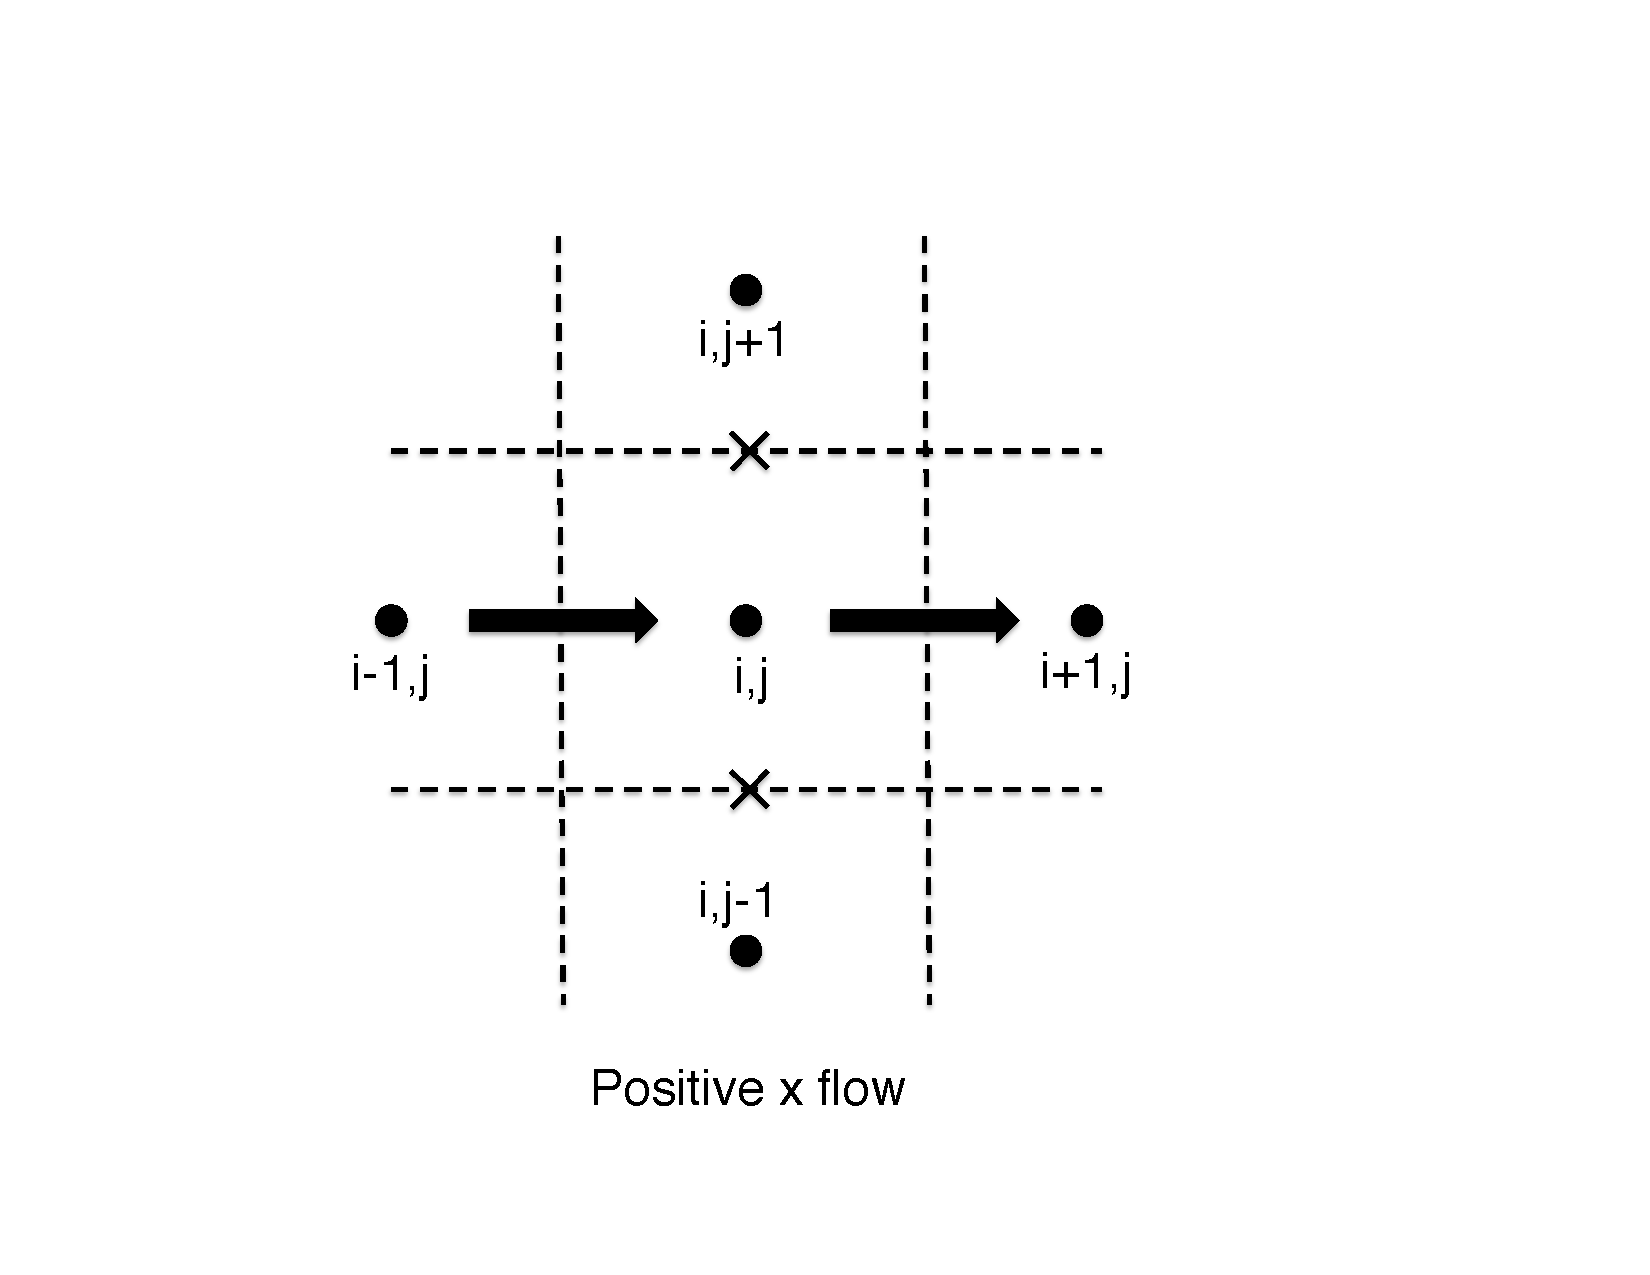
\includegraphics[width=3.0in]{figures/gridposflow.pdf} & 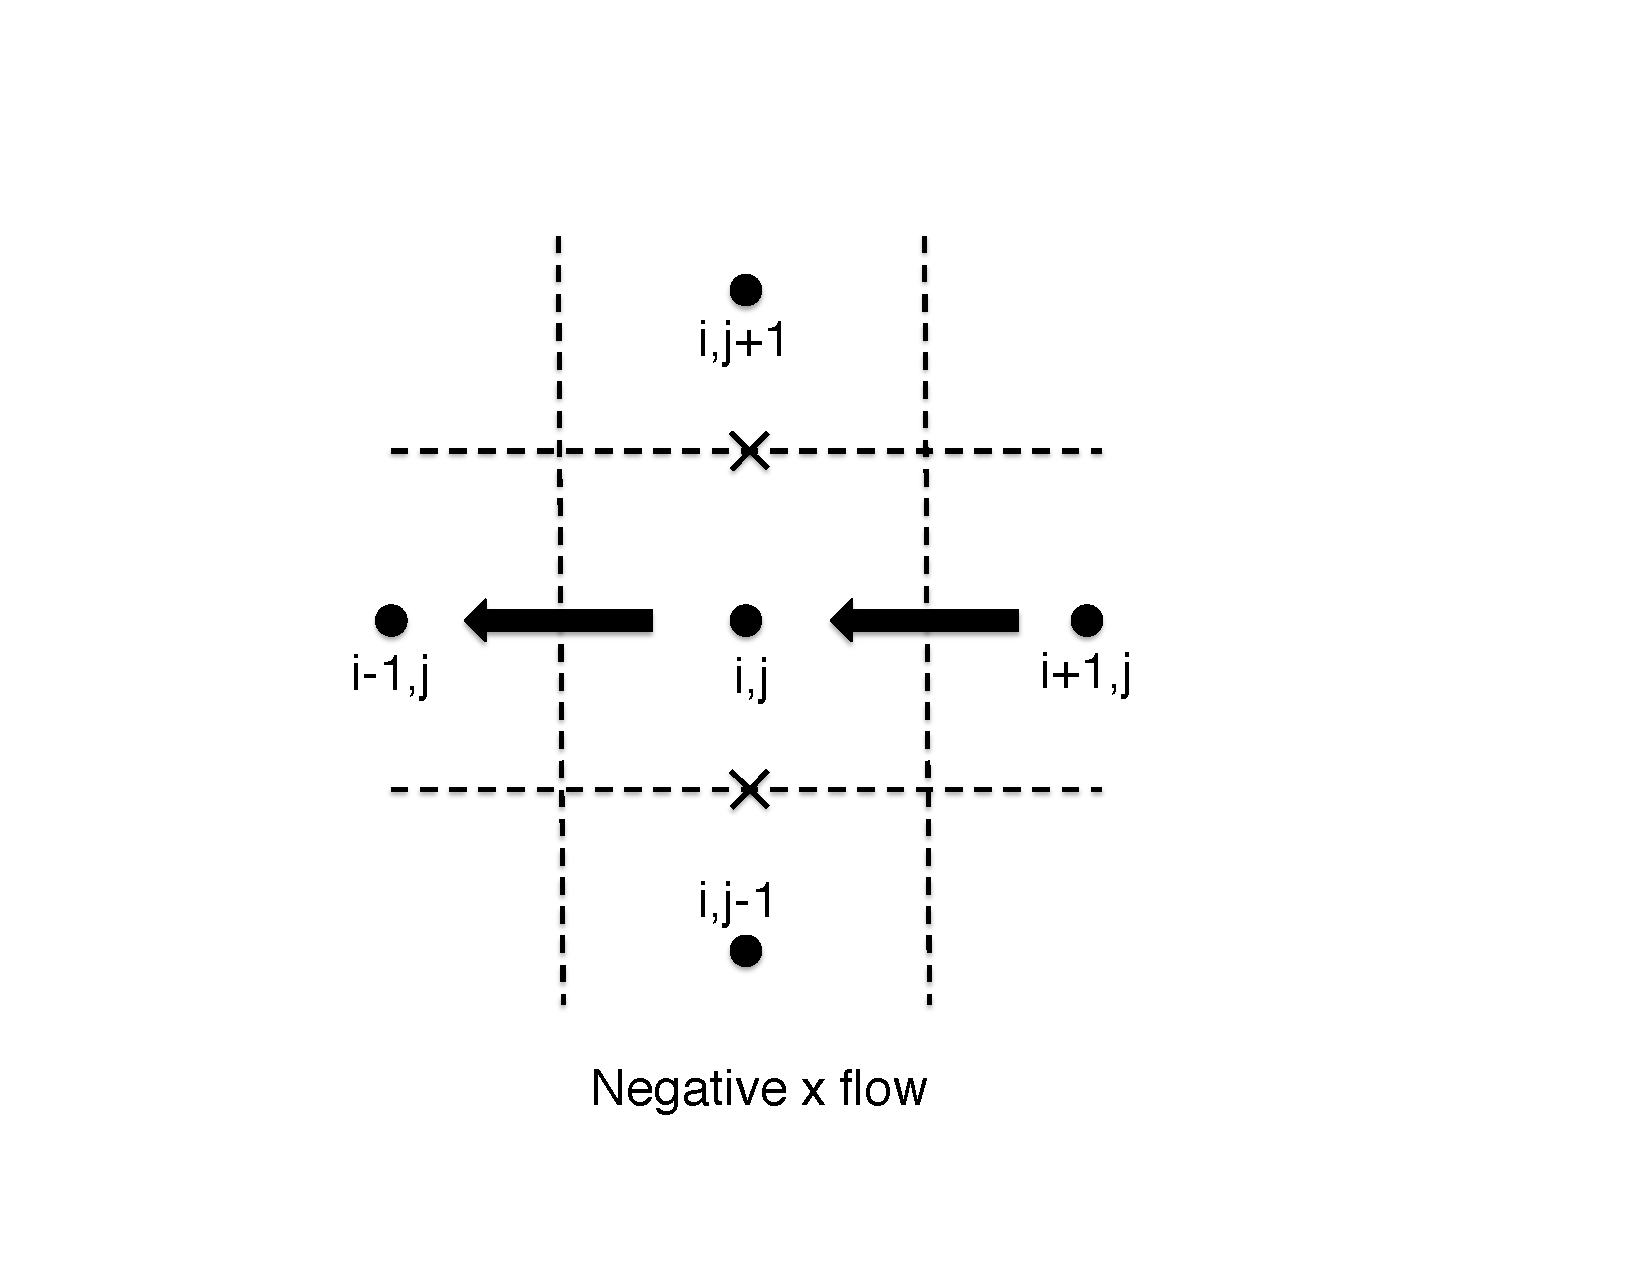
\includegraphics[width=2.77in]{figures/gridnegflow.pdf}
		\end{tabular}
	\end{center}
\end{figure}

Suppose first that $u_{i+1/2,j} > 0$ and $u_{i-1/2,j}>0$; i.e. the velocity in the $x$ direction is positive through cell $ij$ (see Fig.~\ref{flow} left panel). The $x$ contribution to $(\nabla \cdot \bF)_{ij}$ is:
\bee{
\frac{f_{i+1/2,j} - f_{i-1/2,j}}{\Delta x} = \frac{1}{2\Delta x} \left( \left( u_{ij} + u_{i+1,j} \right) C_{ij} -  \left( u_{i-1,j} + u_{i,j} \right)C_{i-1,j}\right). \label{fij}
}
Now let's consider what contributions occur in the adjacent cells under these assumptions. In the $(i+1,j)$-th cell, we know that the flow at the left is positive, which determines the second of the two $x$ terms in Eq.~\eqref{consup}:
\baas{
\frac{- f_{(i+1)-1/2,j}}{\Delta x} &=& -\frac{1}{2\Delta x}\left( u_{(i+1)-1,j} + u_{i+1,j} \right)C_{(i+1)-1,j} \\
&=& -\frac{1}{2\Delta x}\left( u_{ij} + u_{i+1,j} \right)C_{ij}.
}
Notice that this term cancels out the first term in Eq.~\eqref{fij}. Now on the other side, in the $(i-1,j)$-th cell, we know that the flow at the right is positive, which gives us
\baas{
\frac{f_{(i-1)+1/2,j}}{\Delta x} &=& \frac{1}{2\Delta x}\left( u_{i-1,j} + u_{(i-1)+1,j} \right)C_{i-1,j},
}
and cancels the second term in Eq.~\eqref{fij}. 

To summarize, in positive flow the terms at the right edge of cell $ij$ and the left edge of cell $(i+1,j)$ cancel, as do the terms at the left edge of cell $ij$ and the right edge of cell $(i-1,j)$:
\baas{
f_{i+1/2,j} - f_{(i+1)-1/2,j} &=& 0 \\
- f_{i-1/2,j} + f_{(i-1)+1/2,j} &=& 0. 
}
It is not difficult to show the same cancellation in negative flow (Fig.~\ref{flow}, right panel). Since the same terms always cancel regardless of flow direction, no concentration is lost even when the flow directions are opposed coming into the cell. Similar results hold for $g$ in the $y$ direction, so we have demonstrated that this upwinding scheme is conservative.

\section{Nonconservative upwinding}

An example of nonconservative upwinding uses one-sided derivatives based on the signs of the components of $\bu$ at the cell center:
\bees{
(\nabla \cdot \bF)_{ij} \approx \begin{Bmatrix}\dfrac{f_{ij} - f_{i-1,j}}{\Delta x}, & u_{ij} > 0 \\ \dfrac{f_{i+1,j} - f_{ij}}{\Delta x}, & u_{ij} \leq 0 \end{Bmatrix} +  \begin{Bmatrix}\dfrac{g_{ij} - g_{i,j-1}}{\Delta y}, & v_{ij} > 0 \\ \dfrac{g_{i,j+1} - g_{ij}}{\Delta y}, & v_{ij} \leq 0 \end{Bmatrix} .
}
[Add proof of no conservation.]


 
\end{document}